\documentclass{article}
\usepackage[utf8]{inputenc}
\usepackage{graphicx}
\usepackage{setspace}
\usepackage{subcaption}

\title{

\textbf{
    \Huge{DAIICT}\\
    \huge{Gandhinagar}\\
    \huge{Batch ‘24}\\
    \vspace{1cm}
    \LARGE{Academic Year 2020-21}\\\\
    \Huge{SC-205 PROJECT}\\
    \LARGE{END-SEM Project}\\\\
} }


\author
{
    \textit{ \textbf{ \large{-Made by combined efforts of:} } }\\\\
    \textit{ \textbf{ \LARGE{Suyash Vyas \ \ - 202001002} } }\\\\
    \textit{ \textbf{ \LARGE{Praneet Shroff - 202001004} } }\\\\
    \textit{ \textbf{ \LARGE{Vihar Shah \ \ \ \ - 202001110} } }\\\\
    \textit{ \textbf{ \LARGE{Rushabh Patel - 202001419} } }\\\\
}
\date{ \textbf{ \Large{July, 2021} } }

\begin{document}

\pagenumbering{arabic}

\begin{figure}[t]
\centerline{ 
\includegraphics[scale=0.41]{DAIICT_logo.png} }
\label{fig}
\end{figure}

\maketitle

\begin{center}
\underline{\textbf{{\Huge HUFFMAN CODING}}}
\end{center}
\vspace{1cm}

\textbf{ \Large{Assigned By: \\
Professor Manish Gupta \\
Professor Rahul Muthu} }\ \ \ \	



\vspace{2cm}

\begin{center}
\textbf{\Large Abstract\\}

\Large{In the corresponding report, we have tried to explore and implement one 
of the most efficient and trending worldwide method of source 
encoding named as Huffman coding and even focussed 
on its usability and application in real life.\\}
\end{center}

\vspace{1.2cm}

\section{Introduction}

\Large{The source coding concept is very well discussed topic across the globe where researchers are constantly putting their efforts to make the process data efficient and cost-effective at the same time. Even in one of courses of Communication - Introduction to Communication System, we were taught regarding the data transfer, encoding and decoding at the transmitter and receiver end respectively. Thus, it was quite fascinating for us to deep dive into it and code a program which uses the concept of mathematics in order to solve the algorithm and thus execute one of the best known and most compressible form of the data encoding.}\\

\vspace{1cm}

\section{The Formal Statement of the Problem}

\Large{The encoding process can be done for all characters (alphabets, numeric, Greek symbols) with the help of normal decoding, i.e., by assigning a codeword for every unique character and then transmit it, e.g., assuming that there are 6 unique characters. Thus, the codeword used for transmission of each alphabet would comprise a total of 3 binary digits. Let’s write the codeword for few of them}\\ \\
$X1 = 000$\\
$X2 = 001$\\
$X3 = 011$\\
$X4 = 100$\\
$X5 = 101$\\
$X6 = 110$\\

\Large{Thus, during the transmission of a string of 100 characters, we would require a total of 3*100 = 300 bits to be transferred, with an average of 3 bits per character.\\ \\
So, in order to reduce the number of bits transfer, we use the concept of Huffman Coding which is an algorithm that takes as input the frequencies (which are the probabilities of occurrences) of symbols in a string and produces as output a prefix code that encodes the string using the fewest possible bits, among all possible binary prefix codes for these symbols. \\ \\
In simple words it makes codewords with respect to the frequency of occurrence, since more frequent characters have shorter codewords, the bits require to transmit the data will eventually decrease.} \\

\vspace{1cm}

\section{What is Huffman Coding?}

\Large{A MIT graduated scientist David Huffman created an algorithm to compress the data by using the Greedy-choice property and Optimal substructure. The algorithm that takes the frequency of symbols (probability of occurrences) and produces as output a prefix code* that encodes the input string in lowest possible bits.\\ \\
An example of Huffman coding is illustrated below:
}

\begin{center}
\begin{tabular}{| c | c | c | c | c |} 
  
  \hline
  Symbol & Probability /
Frequency
 & Codeword & Length  & Product  \\ 
  \hline
  $X1$ & 0.45 & 0 & 1 & 0.45 \\ 
  \hline
  $X2$ & 0.2 & 111 & 3 & 0.6 \\
  \hline
  $X3$ & 0.13 & 110 & 3 & 0.39 \\
  \hline
  $X4$ & 0.1 & 100 & 3 & 0.3 \\
  \hline
  $X5$ & 0.07 & 1011 & 4 & 0.28 \\
  \hline
  $X6$ & 0.05 & 1010 & 4 & 0.2 \\
  \hline
  
\end{tabular}
\end{center}
\\
\Large{Here we can clearly observe that the sum of the product column is \\
$0.45 + 0.6 + 0.39 + 0.3 + 0.28 + 0.2 = 2.2$ \\ \\
This indicates the average number of bits required which is less than 3 bits which would be consumed as seen before method.\\ \\
}
\small{*  Prefix code is a property where no bit string corresponds to more than one sequence of letters is to encode letters so that the bit string for a letter never occurs as the first part of the bit string for another letter.\\

e.g. - $ x1 = 1, x2 = 00, x3 = 01, x4 = 10$\\

so here the prefix code property is violated and thus it will create errors while decoding, i.e., for an output of 001001 we can have multiple possibilities of the input code, it can be $x2x1x2x1$ or $x2x4x3$.}\\

\vspace{1cm}

\section{The Mathematics behind Huffman Coding:} 

\vspace{.4cm}

\Large{This algorithm uses the concept of a data structure called “Binary Trees” to be more precise “min Heaps”. \\ \\
Rooted Binary Tree – It is a type of graph which have a rode node which acts as the source for a maximum of two branches, left subtree and right subtree. The subtrees can further be grown recursively to produce a huge binary tree / forest, comprising of multiple branches and multiple nodes. \\ \\
Heap – It is a complete binary tree, which means that the tree is completely filled on all levels except possibly the lowest, which is filled from the left up to a point. \\ \\
Thus, for the Huffman coding the following algorithm is implemented: \\

We assume that C is a set of n characters and that each character $c \in C$ is an object with an attribute c.freq giving its frequency. The algorithm builds the tree T corresponding to the optimal code in a bottom-up manner. It begins with the set of $|C|$ leaves and performs a sequence of $|C| - 1$ “merging” operation to create a final tree. The algorithm uses the minimum priority queue Q, keyed on the freq attribute, to identity the two least frequent objects to merge together. When we merge two objects, the result is a new object whose frequency is the sum of the frequencies of the two objects that were merged. The merging of the least frequency leaves continues till there tree is only left with 3 nodes, which will be the left leaf, right leaf and the sum of the left leaf and the right leaf as the root.
}

\vspace{1cm}

\section{Solving the Problem:}

\Large{Pseudocode for HUFFMAN (C): 
\begin{enumerate}
\item $n = |C|$
\item $Q = C$
\item for $i = 1$ to $n-1$
\begin{center}
allocate a new node z \\
z.left = x = EXTRACT-MIN (Q) \\
z.right = y = EXTRACT-MIN (Q) \\
z.freq = x.freq + y.freq \\
\end{center}
\item INSERT (Q, z)
\item return EXTRACT-MIN(Q)
\end{enumerate}

\vspace{.4cm}

By solving the above pseudocode, we created the codewords for the corresponding input string and taking into account the probability/ frequency of the alphabets. We considered the following frequency data.
}

\begin{figure}[ht]
\centering
\begin{subfigure}{.6\textwidth}
  \centering
  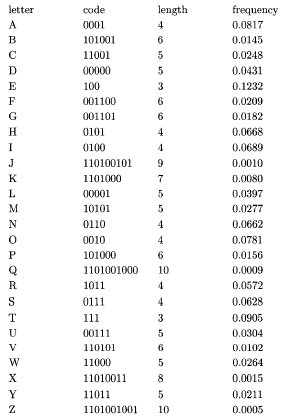
\includegraphics[width=1\linewidth]{P1.png}
  \caption{Courtesy – Discrete Mathematics and Its Application, By Kenneth. H. Rosen \\ \\
  **The Values of Frequency may change as per the internet source  }
  \label{fig:sub1}
\end{subfigure}%
\begin{subfigure}{.38\textwidth}
  \centering
  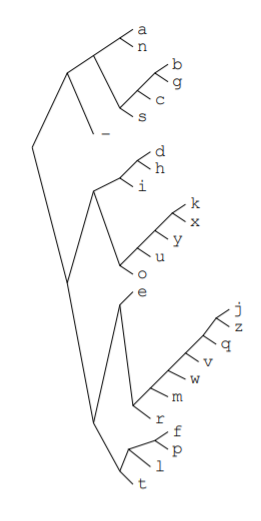
\includegraphics[width=1.1\linewidth]{P2.png}
  \caption{Courtesy – Information Theory,Inference, and learning Algorithm by David. C. Mackay }
  \label{fig:sub2}
\end{subfigure}
\end{figure}

\Large{Thus, by implementing the above pseudocode we coded the program which takes the input as a string from the user and implements the above stated algorithm and the data of frequency and make convert each character into a codeword and displays it as a result. Further it appends all the codewords and generates an encoded message which is ready to be transmitted.}

\vspace{1cm}

\section{The significance of Discrete Mathematics }

\subsection{Time complexity:}

\Large{If there are n nodes, EXTRACT-MIN () is called $2*(n – 1)$ times. EXTRACT-MIN () takes $O(logn)$ time. Thus, a total time of $O(nlogn)$ where n is the number of unique characters. }

\subsection{B.	Trees:}

\Large{It constructs efficient algorithms for locating items in a list, even it helps determine the computational complexity of algorithms based on a sequence of decisions, such as sorting algorithms, thus is make it easy to transverse through the characters input sort the character with least frequency/ probability, even because of dynamic memory allocation, it uses less space in order to compute the algorithm and thus saves times and memory space.}

\vspace{1cm}

\section{Implementation and Significance of the application of the solution}

\Large{Huffman codes compress data very effectively, saving of 20\% to 90\% are typical, depending on the characteristic of the data being compressed. It is currently one of the best algorithms for channel encoding process and there is no better algorithm.}

\vspace{1cm}

\section{MATHEMATICAL APPROACH}

\Large{We have made use of  Binary trees in order to assign code-words to characters, where with each new level in the tree we add 1 to the length of the codewords assigned.}

\begin{figure}[ht]
\centerline{ 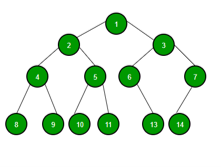
\includegraphics[width=.8\linewidth]{P3.png} }
\label{fig}
\end{figure}
\\

\Large{
Also in order to calculate how often each character is bound to come up we have calculated its probability.\\ \\
Prefix free codes have been used  (using them creates no ambiguity while decoding) \\ \\
\underline{\textbf{Prefix free code:}} \\ 
Codewords which fulfill the prefix free condition are called prefix codes. \\
Any one codeword of a system of codewords cannot be a prefix for a other codeword of the same system. \\
Example: 
\begin{center}
A: 00 \\
B: 010 \\
C: 110 \\
D: 10 \\
\end{center}

We can see that the codeword for A which is 00 is prefix to no other codeword in the list. This is called prefix free code and it helps decode the characters without any ambiguity. \\ \\
\underline{Why is prefix code used here?} \\ 
Basically it helps tackle ambiguity at the time of decoding. Lets understand tat with the help of an example: Say E was also an character in the list with the codeword 0001 then as soon as the compiler would read the birst two bits 00 it would think we are referring to the character A which causes errors at the time of decoding.
}

\vspace{1cm}

\section{COMMERCIALIZATION SCOPE}

\Large{

\begin{itemize}

  \item Huffman Coding technique is currently used over the world for encoding data as it comprises efficiently and thus reduces the amount of data transfer . Due to the lack of patent coverage, simplicity and speed, prefix codes are widely used. So it can be used to create a data compression service, that on the surface would be free but still make money through ads. \\ 

\item Huffman coding  is not used directly in real world but several derivatives of Huffman encoding algorithm is used in application like JPEG, PNG, MP3 etc. It can be implemented in combination with these compression techniques to compress variety of data like images, music, video files. \\ 

\item It can also be used to create an encryption service, if we use as the key a probability distribution then we can create Huffman codes for each characters that  can be used to encrypt them (But we will be trading off the compression for encryption). \\ \\

\end{itemize}

Now where would such encryption finds it use? There is a pretty well knows way some people use to crack the key and that is ‘Brute force’ method, so if we Huffman encode a text before encrypting it, the attacker would not only has to decrypt the text but also Huffman decode it to get to the password.
}

\end{document}